\documentclass[letterpaper,12pt]{article}

%%%%%%%%%%%%%%%%%%%%%%%% Standard Packages %%%%%%%%%%%%%%%%%%%%%%%%%%%%%%%%%%%%%%%%%%
\usepackage{epsfig}
\usepackage{graphicx}
\usepackage{graphics}
\usepackage{amssymb}
\usepackage{amsmath}
\usepackage{fancyvrb}
\usepackage{comment}
\usepackage{fancyhdr}
\usepackage{color}
\usepackage{amsfonts}

%%%%%%%%%%%%%%%%%%%%%%%% Adapted from Sweave %%%%%%%%%%%%%%%%%%%%%%%%%%%%%%%%%%%%%%%%%
\DefineVerbatimEnvironment{Rcode}{Verbatim}{fontshape=sl, frame=single, 
  framesep=2mm, fontsize=\small, baselinestretch=.5}

%%%%%%%%%%%%%%%%%%%%%%%% Page and Document Setup %%%%%%%%%%%%%%%%%%%%%%%%%%%%%%%%%%%%%
\addtolength{\oddsidemargin}{-0.875in}
\addtolength{\topmargin}{-0.875in}
\addtolength{\textwidth}{1.75in}
\addtolength{\textheight}{1.75in}

\renewcommand{\topfraction}{0.9}        % max fraction of floats at top
\renewcommand{\bottomfraction}{0.8}     % max fraction of floats at bottom

% Parameters for TEXT pages (not float pages):
\setcounter{topnumber}{2}
\setcounter{bottomnumber}{2}
\setcounter{totalnumber}{4}             % 2 may work better
\setcounter{dbltopnumber}{2}            % for 2-column pages
\renewcommand{\dbltopfraction}{0.9}     % fit big float above 2-col. text
\renewcommand{\textfraction}{0.07}      % allow minimal text w. figs

% Parameters for FLOAT pages (not text pages):
\renewcommand{\floatpagefraction}{0.7}          % require fuller float pages

% N.B.: floatpagefraction MUST be less than topfraction !!
\renewcommand{\dblfloatpagefraction}{0.7}       % require fuller float pages


\def\argmax{\operatornamewithlimits{arg\,max}}
\def\argmin{\operatornamewithlimits{arg\,min}}

\definecolor{myblue}{rgb}{0.25, 0, 0.75}
\definecolor{mygold}{rgb}{1,0.8,0.2}
\definecolor{gray}{rgb}{0.5, 0.5, 0.5}

\newcommand{\myurl}[1]{\href{http://#1}{\textcolor{gray}{\texttt{#1}}}}
\newcommand{\myem}[1]{\structure{#1}}
\newcommand{\myurlshort}[2]{\href{http://#1}{\textcolor{gray}{\textsf{#2}}}}

\newcommand{\RPackage}[1]{\textcolor{gray}{\textsf{#1}}}
\newcommand{\PL}[1]{\texttt{#1}}
\newcommand{\RCode}[1]{\texttt{#1}}
\newcommand{\RFunction}[1]{\textsf{#1}}
\newcommand{\RClass}[1]{\textcolor{mygold}{\textsf{#1}}}
\newcommand{\BIOCfunction}[1]{\textcolor{orange}{#1}}

%%%%%%%%%%%%%%%%%%%%%%% options for sweave %%%%%%%%%%%%%%%%%%%%%%%%%%%%%%%%%%%%%%%%%%%%


%%%%%%%%%%%%%%%%%%%%%%% headers and footers %%%%%%%%%%%%%%%%%%%%%%%%%%%%%%%%%%%%%%%%%%%
\pagestyle{fancy} 
\renewcommand{\footrulewidth}{\headrulewidth}

%%%%%%%%%%%%%%%%%%%%%%% bibliography %%%%%%%%%%%%%%%%%%%%%%%%%%%%%%%%%%%%%%%%%%%%%%%%%%
\bibliographystyle{plainnat}

%%%%%%%%%%%%%%%%%%%%%%% opening %%%%%%%%%%%%%%%%%%%%%%%%%%%%%%%%%%%%%%%%%%%%%%%%%%%%%%%
\title{DNA-Modification Detection with SMRT-Sequencing using R}
\author{Pacific Biosciences}

\usepackage{Sweave}
\begin{document}
\maketitle

\section{Introduction}
\subsection{Samples Analyzed}
\subsection{R Packages}
\subsection{Experimental Design}

\section{Exploring the Data}
As described above, SMRT-Sequecing provides a rich set of information
beyond that of traditional sequencing platforms. Specifically, here we
focus on information about the kinetic behavior of the polymerase at
specific positions in the reference sequence. We first examine
high-level summaries of the data, such as yield, read length, and
accuracy. We will focus on the Lambda data for these analyses, and to
back to the synthetic data for test validation.

\subsection{Working with the Compare H5 File}
The cmp.h5 file (pronounced comp H5 or compare H5) provides a rich set
data resulting from the alignments of Pac Bio data to a reference
sequence. The cmp.h5 file may contain one or more movies and contains
all of the alignments for that movie's reads to a reference fasta
file.
\begin{Schunk}
\begin{Sinput}
> require(pbh5)
> require(pbutils)
> require(ggplot2)
> files <- list.files("../Data/Lambda", pattern = "6ma*", full.names = T)
> names(files) <- basename(files)
> cmpH5 <- PacBioCmpH5(paste(files[1], "data", "aligned_reads.cmp.h5", 
+     sep = "/"))
> refGroup(cmpH5)
\end{Sinput}
\begin{Soutput}
  RefInfoID ID       Path offsetBegin offsetEnd      Name       FullName Length
1         1  1 /ref000001           1    149408 ref000001 lambda_NEB3011  48502
                               MD5
1 a1319ff90e994c8190a4fe6569d0822a
\end{Soutput}
\end{Schunk}
The alignments, along with all of the relevant kinetics data, are
stored in a directory like structure corresponding to their reference
and movie, e.g.,
\begin{Schunk}
\begin{Sinput}
> rGroup <- "ref000001/m110818_075520_42141_c100129202555500000315043109121112_s1_p0"
> g <- getH5Group(cmpH5, rGroup)
> ls(g)
\end{Sinput}
\begin{Soutput}
[1] "."            "AlnArray"     "DeletionQV"   "IPD"          "InsertionQV" 
[6] "PulseWidth"   "QualityValue"
\end{Soutput}
\end{Schunk}
Each of the datasets stored here represent all of the alignments for
a given movie. For our work, the most pertinent datasets are:
AlnArray, IPD (inter-pulse duration), and PulseWidth. The IPD and
PulseWidth describe kinetic properties of the sequencing and the
AlnArray will tell us which base we are incorporating.

All of the alignments in the file are stored in a global alignment
index, which can be accessed as follows:
\begin{Schunk}
\begin{Sinput}
> head(alnIndex(cmpH5), 2)
\end{Sinput}
\begin{Soutput}
     ID
1 93787
2 74915
                                                              alnGroupPath
1 /ref000001/m110818_075520_42141_c100129202555500000315043109121112_s1_p0
2 /ref000001/m110818_075520_42141_c100129202555500000315043109121112_s2_p0
                                                      movieName   refName
1 m110818_075520_42141_c100129202555500000315043109121112_s1_p0 ref000001
2 m110818_075520_42141_c100129202555500000315043109121112_s2_p0 ref000001
     fullRefName tStart tEnd alignedStrand holeNumber setNumber strobeNumber
1 lambda_NEB3011      1   89             0      22178         1            0
2 lambda_NEB3011      1   97             1      17892         2            0
  moleculeID rStart rEnd mapQV nMatches nMisMatches nInsertions nDeletions
1     342178    278  381   254       87           0          17          2
2     657892   3520 3625   254       93           4           9          0
  offsetBegin offsetEnd nBackRead nOverlap
1     4542502   4542607         0        0
2    25681054  25681159         1        1
\end{Soutput}
\end{Schunk}
or more succinctly, 
\begin{Schunk}
\begin{Sinput}
> head(cmpH5, 2)
\end{Sinput}
\begin{Soutput}
     ID
1 93787
2 74915
                                                              alnGroupPath
1 /ref000001/m110818_075520_42141_c100129202555500000315043109121112_s1_p0
2 /ref000001/m110818_075520_42141_c100129202555500000315043109121112_s2_p0
                                                      movieName   refName
1 m110818_075520_42141_c100129202555500000315043109121112_s1_p0 ref000001
2 m110818_075520_42141_c100129202555500000315043109121112_s2_p0 ref000001
     fullRefName tStart tEnd alignedStrand holeNumber setNumber strobeNumber
1 lambda_NEB3011      1   89             0      22178         1            0
2 lambda_NEB3011      1   97             1      17892         2            0
  moleculeID rStart rEnd mapQV nMatches nMisMatches nInsertions nDeletions
1     342178    278  381   254       87           0          17          2
2     657892   3520 3625   254       93           4           9          0
  offsetBegin offsetEnd nBackRead nOverlap
1     4542502   4542607         0        0
2    25681054  25681159         1        1
\end{Soutput}
\end{Schunk}
To access an alignment or data associated with an alignment, we will
use accessor functions which take a cmp.h5 file as well as a vector of
indices refering to the rows in the alignment index which we want to
retrieve.
\begin{Schunk}
\begin{Sinput}
> alns <- getAlignments(cmpH5, 1:3)
> sapply(alns, nrow)
\end{Sinput}
\begin{Soutput}
[1] 106 106 116
\end{Soutput}
\begin{Sinput}
> head(alns[[1]])
\end{Sinput}
\begin{Soutput}
     read reference
[1,] "G"  "G"      
[2,] "G"  "G"      
[3,] "G"  "G"      
[4,] "C"  "C"      
[5,] "G"  "G"      
[6,] "G"  "G"      
\end{Soutput}
\end{Schunk}
The above command retrieves the first 3 alignments, 

\section{Normalization}



\section{Statistical Testing}
In this section we focus on two-sample statistical tests comparing the
IPD distribution in a control sample to a treatment. Each particular
DNA modification has a different signature at or around the modified
base and more sophisticated methods will take that into account. In
this section, we will first focus on the Synthetic data sets where the
modified positions are known. Here, we will look at detection as a
function of coverage. In general, with sufficient coverage the
difference between IPD distributions can be detected, however, certain
modifications do not have a large effect on the kinetics of the
polymerase and therefore to detect these smaller effects we need to
observe the incorporation event many times.

\begin{Schunk}
\begin{Sinput}
> cmpH5s <- lapply(Sys.glob("../Data/Synthetic/*/data/aligned_reads.cmp.h5"), 
+     PacBioCmpH5)
> names(cmpH5s) <- sapply(cmpH5s, function(h) basename(dirname(dirname(h@fileName))))
> modifications <- list(`2x_5mC` = c(55, 74), `2x_5hmC` = c(51, 
+     74), `2x_4mC` = c(55, 74), `2x_6mA` = c(57, 68))
\end{Sinput}
\end{Schunk}

We now define a testing function which represents a number of choices
in the analysis via its parameterization.
\begin{Schunk}
\begin{Sinput}
> testPositions <- function(treatmentH5, controlH5, testStatistic = wilcox.test, 
+     targetStrands = c(0, 1), targetPositions = NA, targetCoverage = c(10, 
+         50, 100, 500, 1000), getData = getByTemplatePosition, 
+     whReference = 1) {
+     if (any(is.na(targetPositions))) {
+         start <- 1
+         end <- refInfo(controlH5)$Length[whReference]
+     }
+     else {
+         start <- min(targetPositions)
+         end <- max(targetPositions)
+     }
+     tReads <- getReadsInRange(treatmentH5, whReference, start, 
+         end)
+     cReads <- getReadsInRange(controlH5, whReference, start, 
+         end)
+     tData <- getData(treatmentH5, idx = tReads)
+     cData <- getData(controlH5, idx = cReads)
+     tData <- subset(tData, (strand %in% targetStrands) & (position >= 
+         start & position <= end) & read == ref)
+     cData <- subset(cData, (strand %in% targetStrands) & (position >= 
+         start & position <= end) & read == ref)
+     g <- function(v, n) {
+         if (length(v) > n) 
+             sample(v, size = n)
+         else v
+     }
+     mapply(function(tIdxs, cIdxs) {
+         lapply(targetCoverage, function(n) {
+             testStatistic(tData$elt[g(tIdxs, n)], cData$elt[g(cIdxs, 
+                 n)])
+         })
+     }, split(1:nrow(tData), factor(tData$position, start:end)), 
+         split(1:nrow(cData), factor(cData$position, start:end)), 
+         SIMPLIFY = FALSE)
+ }
> plotResult <- function(tp, modifiedPositions, g = function(z) -log10(z$p.value), 
+     ...) {
+     par(mfrow = c(5, 1), mar = c(2, 2, 1, 1))
+     sapply(1:5, function(i) {
+         positions <- as.integer(names(tp))
+         y <- sapply(tp, function(x) g(x[[i]]))
+         plot(positions, y, xlab = "", ylab = "", main = "")
+     })
+ }
> testResults <- lapply(cmpH5s[1:4], function(tH5) {
+     testPositions(tH5, cmpH5s$control, targetStrands = 0)
+ })
\end{Sinput}
\end{Schunk}

\begin{Schunk}
\begin{Sinput}
> plotResult(testResults[["2x_5mC"]])
\end{Sinput}
\begin{Soutput}
[[1]]
NULL

[[2]]
NULL

[[3]]
NULL

[[4]]
NULL

[[5]]
NULL
\end{Soutput}
\end{Schunk}
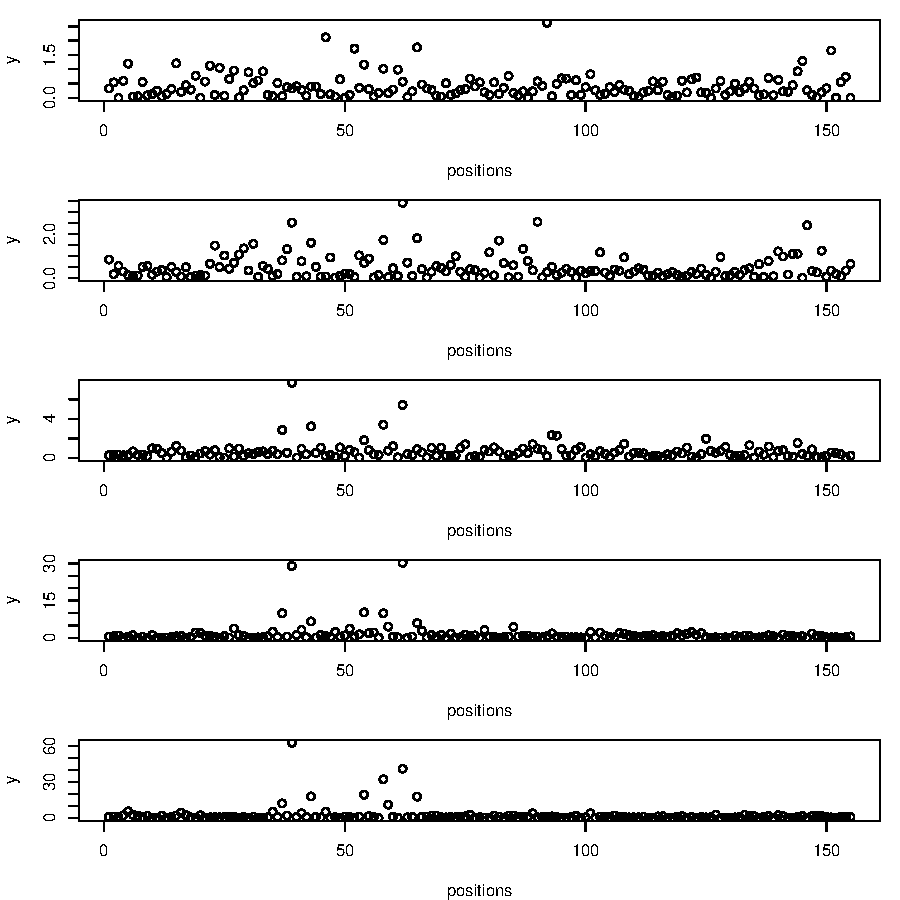
\includegraphics{plots/plots-008}

\begin{Schunk}
\begin{Sinput}
> getIPDForPosition <- function(p) {
+     lapply(cmpH5s[c("2x_5mC", "control")], function(cmpH5) {
+         subset(getByTemplatePosition(cmpH5, idx = sample(1:nrow(cmpH5), 
+             size = 1000)), position == p & strand == 0 & read == 
+             ref)$elt
+     })
+ }
> minPos <- which.min(sapply(testResults[["2x_5mC"]], function(b) b[[5]]$p.value))
> par(mfrow = c(1, 2))
> plotDensity(getIPDForPosition(minPos), legend = T, xlab = "IPD", 
+     log = "x", main = paste("IPD Distributions for position", 
+         minPos))
> plotDensity(getIPDForPosition(15), legend = T, xlab = "IPD", 
+     log = "x", main = paste("IPD Distributions for position", 
+         15))
\end{Sinput}
\end{Schunk}
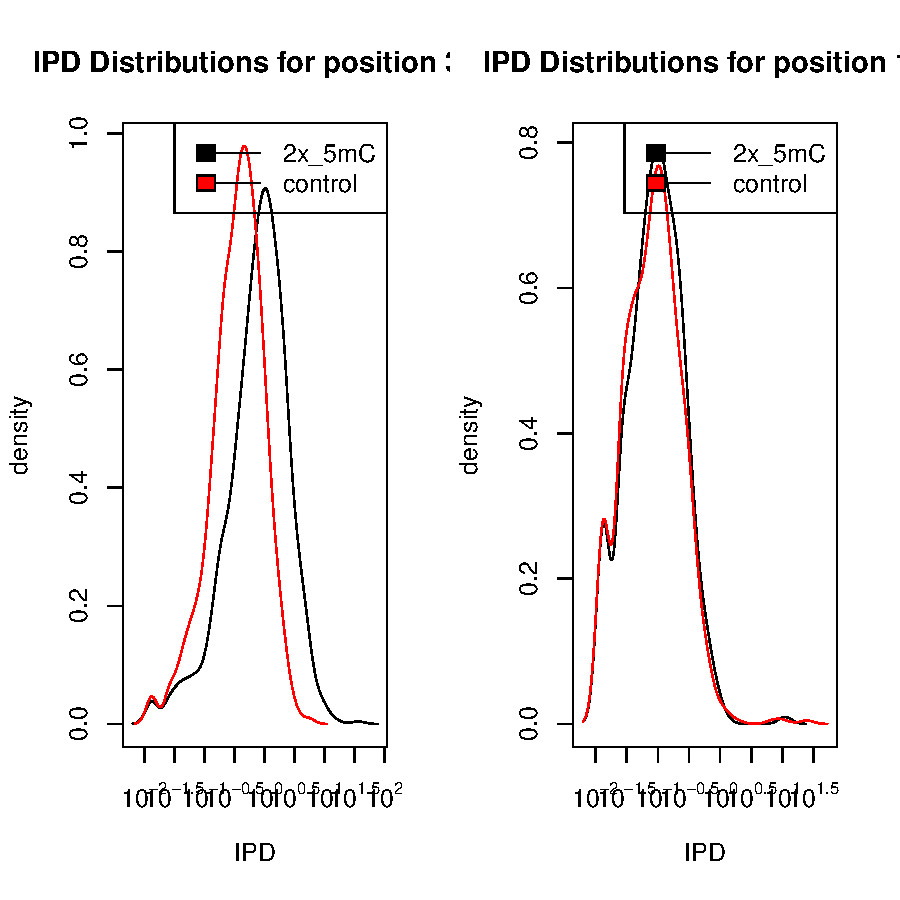
\includegraphics{plots/plots-showDifferentDistributions}

\section{Evaluation}
In this section we evaluate the performance of a statistical test via
ROC analysis. We can determine if a particular testing procedure
outperforms another get a sense of our true-positive rate as well as
our false-positive rate. In this section we focus on just the ``5mC''
condition as it typically demonstrates the smallest effect on the IPD
distributions.
\begin{Schunk}
\begin{Sinput}
> trimmedSlog <- function(x, trim = 0.975, alpha = 1/100) {
+     log(x[x < quantile(x, trim)] + alpha)
+ }
> testFunctions <- list(wilcox.test = wilcox.test, trimmed.slog.t = function(x, 
+     y) {
+     t.test(trimmedSlog(x), trimmedSlog(y))
+ }, permutation.test = function(x, y) {
+     s <- median(x) - median(y)
+     d <- pbutils::collapse(list(x = x, y = y))
+     n <- replicate(500, {
+         diff(tapply(d$value, sample(d$L1), median))
+     })
+     list(statistic = s, p.value = 1 - mean(abs(s) > abs(n)))
+ }, lr.test = function(x, y) {
+     z <- c(lx <- trimmedSlog(x), ly <- trimmedSlog(y))
+     m1 <- sum(dnorm(z, mean(z), sd(z), log = T))
+     m2 <- sum(dnorm(lx, mean(lx), sd(lx), log = T)) + sum(dnorm(ly, 
+         mean(ly), sd(ly), log = T))
+     stat <- -2 * (m1 - m2)
+     list(statistic = stat, p.value = 1 - pchisq(stat, 2))
+ })
> byTestFunction <- lapply(testFunctions, function(f) {
+     testPositions(cmpH5s$"2x_5mC", cmpH5s$control, targetStrands = 0, 
+         testStatistic = f)
+ })
\end{Sinput}
\end{Schunk}

We have 4 different test procedures. We can see immediately that there
are many possible choices in terms of trimming, logging, and the
appropriate null distribution for the test statistic.
\begin{Schunk}
\begin{Sinput}
> truePositives <- rep(FALSE, 155)
> truePositives[c(39L, 58L, 54L, 65L, 59L, 43L, 37L, 35L, 40L, 
+     10L)] <- TRUE
> truePositives <- factor(truePositives, c(TRUE, FALSE))
> roc <- lapply(byTestFunction, function(testRes) {
+     x <- sapply(testRes, function(r) r[[5]]$p.value)
+     do.call(rbind, lapply(c(sort(x), Inf), function(q) {
+         tbl <- table(truth = truePositives, observed = factor(x < 
+             q, c(TRUE, FALSE)))
+         c(tbl[2, 1]/sum(tbl[2, ]), tbl[1, 1]/sum(tbl[1, ]))
+     }))
+ })
> plot(NA, xlim = c(0, 1), ylim = c(0, 1), xlab = "FPR", ylab = "TPR")
> mapply(function(r, col) {
+     points(r[, 1], r[, 2], type = "l", col = col, lwd = 2)
+ }, roc, 1:length(roc))
\end{Sinput}
\begin{Soutput}
$wilcox.test
NULL

$trimmed.slog.t
NULL

$permutation.test
NULL

$lr.test
NULL
\end{Soutput}
\begin{Sinput}
> abline(0, 1, col = "darkgrey", lwd = 2, lty = 3)
> legend("bottomright", names(roc), fill = 1:length(roc))
\end{Sinput}
\end{Schunk}
\includegraphics{plots/plots-011}

\section{Conclusion}

 
\end{document}
